%region : INTELLIJ
\section{Conociendo \textit{IntelliJ}}
  Ahora sí, llegó el momento de la verdad, \textit{Nostradamus} predijo que algún día instalarían
  \textit{IntelliJ}, y ese día es hoy.
  Si eres estudiante, puedes obtener una licencia para utilizar la versión \textit{Ultimate} de
  forma gratuita siguiendo las instrucciones que aparecen en el 
  \href{https://www.jetbrains.com/community/education/#students}{sitio oficial} de 
  \textit{JetBrains}, esto les dará acceso a todas las herramientas de \textit{JetBrains}.

  Para esta parte usaremos como ejemplo la versión \textit{Community}, pero las instrucciones son
  las mismas para la versión \textit{Ultimate}.

  En la figura \ref{fig:jb-toolbox} pueden ver la interfaz de \textit{JetBrains Toolbox}, en este
  caso nos interesa instalar \textit{IntelliJ IDEA Community Edition}.

  \begin{figure}[ht!]
    \centering
    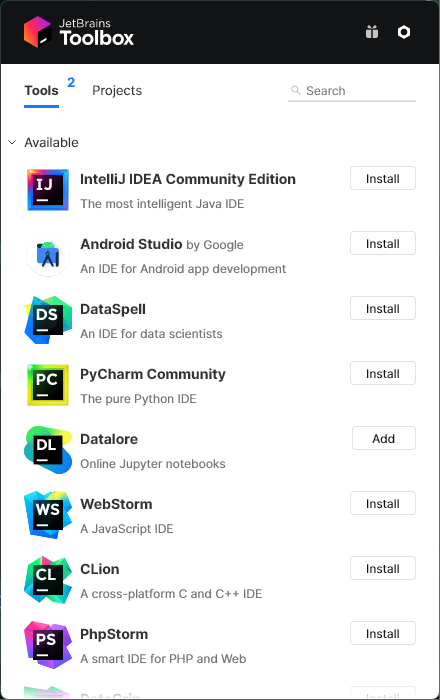
\includegraphics[width=0.4\textwidth]{Por_algo_se_empieza/jetbrains-toolbox.png}
    \caption{Interfaz de \textit{JetBrains Toolbox}.}
    \label{fig:jb-toolbox}
  \end{figure}

  Y eso es todo.
  \textit{IntelliJ} está instalado, ahora vamos a usarlo.

  \subsection{Creando un proyecto}
    El primer paso para utilizar \textit{IntelliJ} es abrirlo (amazing), esto puede tomar varios 
    minutos dado que el \textit{IDE} ocupa muchos recursos.

    Una vez abierto debieran ver una ventana similar a la de la figura \ref{fig:intellij-landing}.
    Aquí deberán seleccionar la opción \enquote{\textit{New Project}}.

    \begin{figure}[ht!]
      \centering
      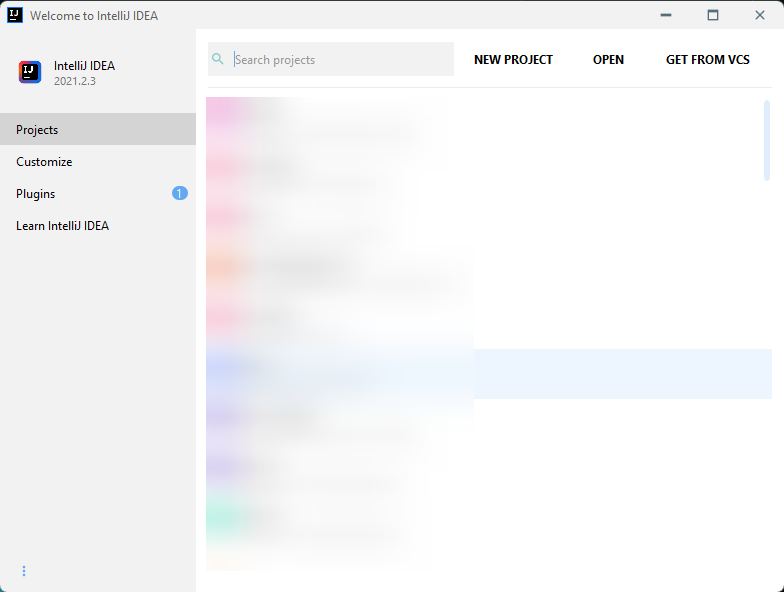
\includegraphics[width=0.5\textwidth]{Por_algo_se_empieza/idea64_HkClRzeuYD.png}
      \caption{Ventana inicial de \textit{IntelliJ}.}
      \label{fig:intellij-landing}
    \end{figure}

    Luego deberíamos estar en la ventana principal de creación de proyectos (figura 
    \ref{fig:intellij-new-project-1}), aquí tendremos muchas opciones disponibles pero en este
    libro las ignoraremos y sólo le pondremos atención a proyectos de \textit{Java} (y 
    posteriormente \textit{Gradle}).
    Si quieren seguir los ejemplos en \textit{Kotlin} deberán marcar la opción resaltada y seguir
    a la siguiente pantalla con \enquote{\textit{Next}}.

    \begin{figure}[ht!]
      \centering
      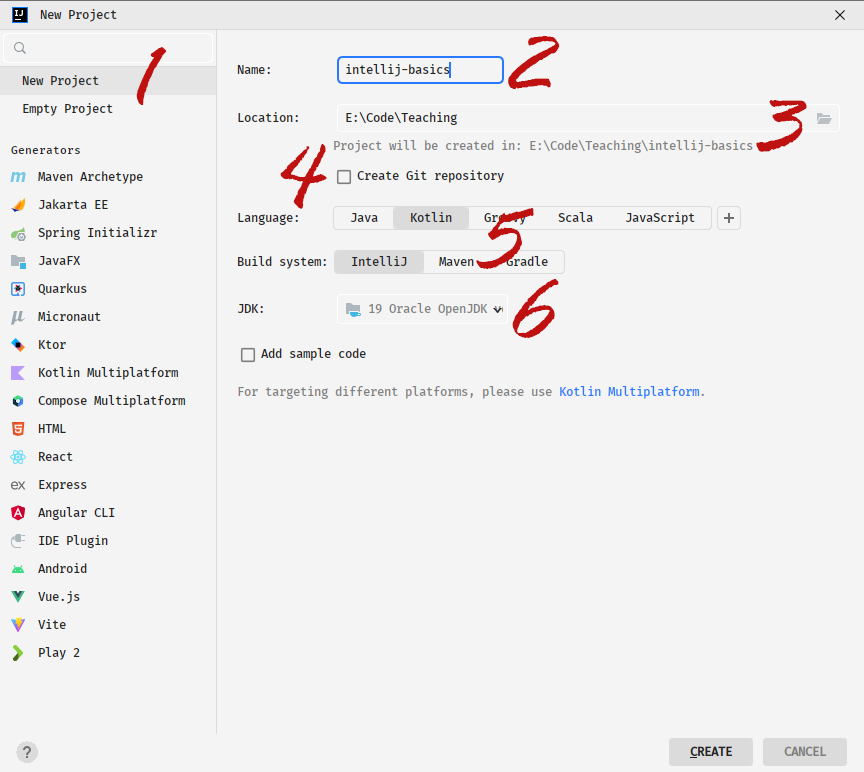
\includegraphics[width=0.7\textwidth]{Por_algo_se_empieza/idea64_new_project_1.png}
      \caption{Ventana de creación de proyectos}
      \label{fig:intellij-new-project-1}
    \end{figure}

    La pantalla siguiente es bastante más simple, aquí definiremos el nombre y la ubicación de 
    nuestro proyecto.
    En este caso lo llamaremos \enquote{IntelliJBasics}.
    Una vez que hayamos terminado, deberíamos finalmente ver la interfaz principal de 
    \textit{IntelliJ} (figura \ref{fig:intellij-main}).

    \begin{figure}[ht!]
      \centering
      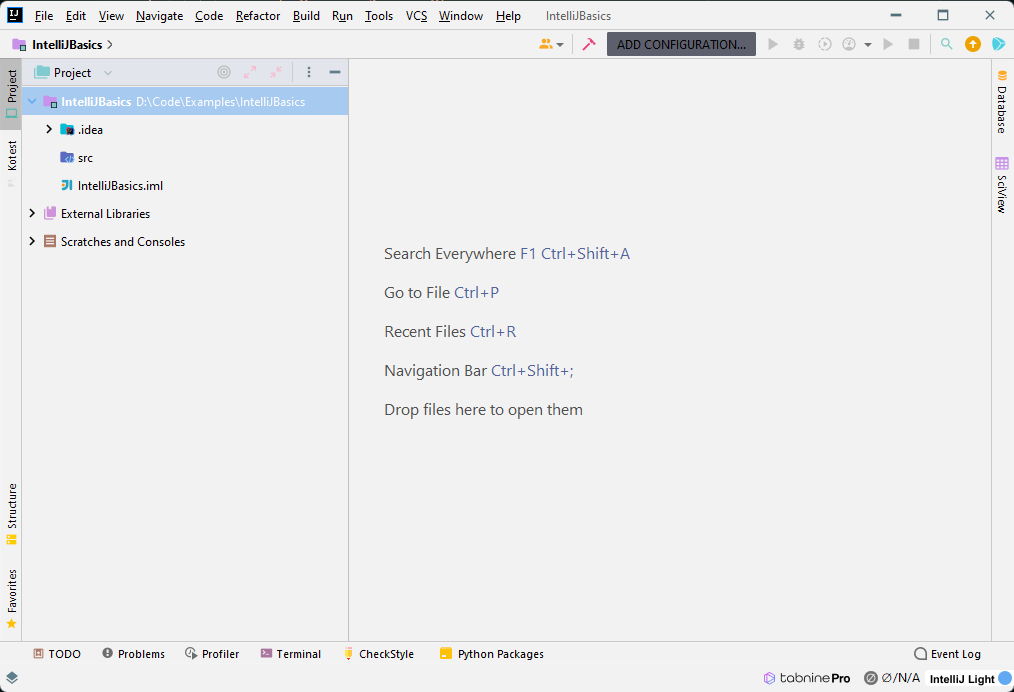
\includegraphics[width=0.6\textwidth]{Por_algo_se_empieza/idea64_main.png}
      \caption{Pantalla principal de \textit{IntelliJ}.}
      \label{fig:intellij-main}
    \end{figure}

    ¡Y listo, tenemos nuestro primer proyecto!

  \subsection{Trabajando con \textit{IntelliJ}}
    En el \cref{ch:java} les dije que nos despediríamos de \textit{jshell}, les mentí
    (parcialmente).
    Antes de comenzar a utilizar realmente \textit{IntelliJ} para crear un programa veremos una
    pincelada de las funcionalidades de este \textit{IDE} mediante la consola de \textit{Jshell}
    de \textit{IntelliJ}.

    Pueden acceder a la consola desde la sección \enquote{Tools} como se muestra en la 
    \cref{fig:tools-jshell}.

    \begin{figure}[ht!]
      \centering
      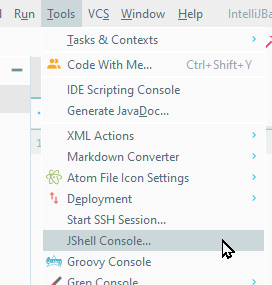
\includegraphics[width=0.4\textwidth]{Por_algo_se_empieza/idea64_tools_jshell.png}
      \caption{Acceso a la consola \textit{JShell}.}
      \label{fig:tools-jshell}
    \end{figure}

    \begin{tcolorbox}[enhanced, breakable, title=\textit{Search Everywere}]
      Otra forma de abrir la consola de \textit{Jshell} es abriendo el menú \textit{Search 
      Everywhere}\footnote{Disponible en todos los \textit{IDEs} de \textit{JetBrains}} 
      (ver \cref{fig:idea64-search-everywhere}), y en la barra de búsqueda escribir 
      texttt{jshell}.

      Esta herramienta nos ayudará mucho a conocer y usar las herramientas de \textit{IntelliJ}.

      \begin{figure}[H]
        \centering
        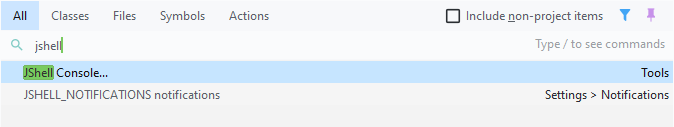
\includegraphics[width=0.7\textwidth]{Por_algo_se_empieza/idea64_search_everywhere.png}
        \caption{Resultado de \textit{Search Everywhere} para la búsqueda de \texttt{jshell}.}
        \label{fig:idea64-search-everywhere}
      \end{figure}
    \end{tcolorbox}

    Ahora intenten reescribir el código de \textit{Java} del \cref{ch:java} para ver cómo se 
    siente trabajar con un \textit{IDE}.
    Deberían tener algo como en la \cref{fig:idea64-jshell-fibonacci}.
    Luego pueden ejecutar el código y ver el resultado en la consola presionando el botón 
    \enquote{\textit{play}} en la esquina superior izquierda del script.

    \begin{figure}[ht!]
      \centering
      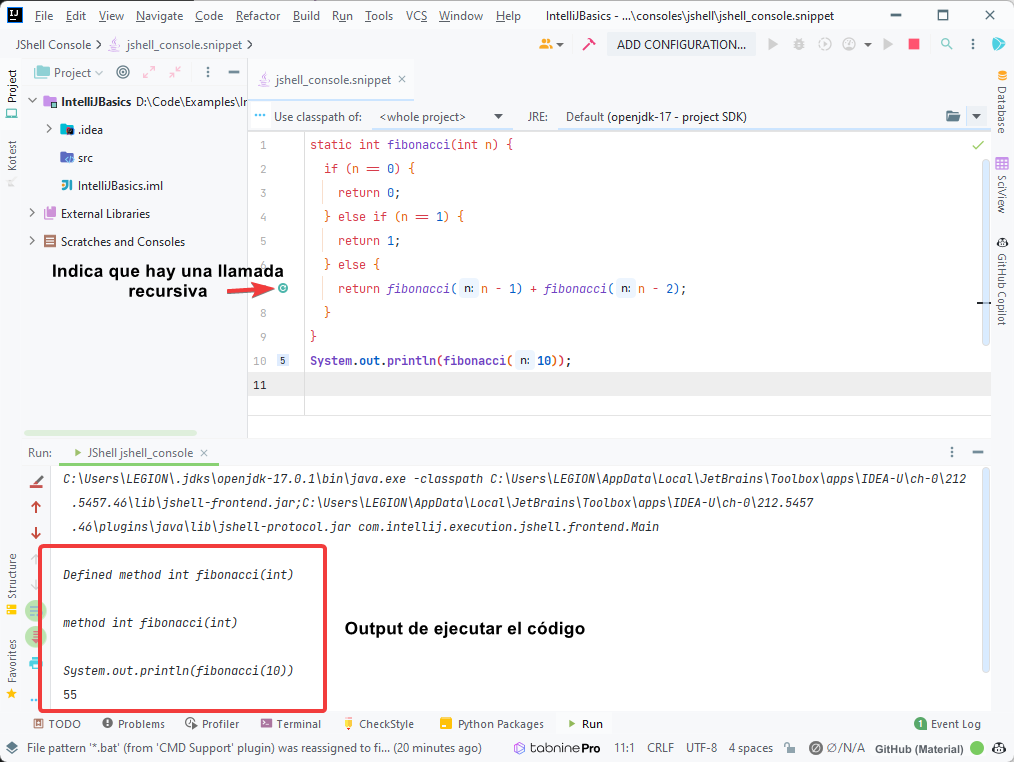
\includegraphics[width=0.9\textwidth]{Por_algo_se_empieza/idea64_jshell_fibonacci.png}
      \caption{Ejemplo de uso de \textit{JShell} en \textit{IntelliJ}.}
      \label{fig:idea64-jshell-fibonacci}
    \end{figure}

    Noten que al definir la función \texttt{fibonacci} agregamos la \textit{keyword}
    \texttt{static} al principio de la función, es complejo explicar la razón de eso en este
    momento, así que por ahora sólo créanme que se hace así.
%endregion